\documentclass[10pt,a4paper,twocolumn,twoside]{article}
\usepackage[utf8]{inputenc}
\usepackage[catalan]{babel}
\usepackage{multicol}
\usepackage{graphicx}
\usepackage{fancyhdr}
\usepackage{times}
\usepackage{titlesec}
\usepackage{multirow}
\usepackage{lettrine}
\usepackage{hyperref}
\usepackage{enumitem}
\usepackage{pgfgantt}
\usepackage{needspace}
\usepackage[top=2cm, bottom=1.5cm, left=2cm, right=2cm]{geometry}
\usepackage[figurename=Fig.,tablename=TAULA]{caption}
\usepackage{apacite}
\captionsetup[table]{textfont=sc}

\hypersetup{
    colorlinks=true,
    linkcolor=black,
    filecolor=black,      
    urlcolor=blue,
    citecolor=black
}

\author{\LARGE\sffamily Narcís Nogué Bonet}
\title{\Huge{\sffamily Aterratge autònom d'aeronaus d'ala fixa basat en visió}}
\date{}

\newcommand\blfootnote[1]{%
  \begingroup
  \renewcommand\thefootnote{}\footnote{#1}%
  \addtocounter{footnote}{-1}%
  \endgroup
}

%
%\large\bfseries\sffamily
\titleformat{\section}
{\large\sffamily\scshape\bfseries}
{\textbf{\thesection}}{1em}{}

\begin{document}

\fancyhead[LO]{\scriptsize NARCÍS NOGUÉ BONET}
\fancyhead[RO]{\thepage}
\fancyhead[LE]{\thepage}
\fancyhead[RE]{\scriptsize ATERRATGE AUTÒNOM D'AVIONS MODEL BASAT EN VISIÓ}

\fancyfoot[CO,CE]{}

\fancypagestyle{primerapagina}
{
   \fancyhf{}
   \fancyhead[L]{\scriptsize TFG EN ENGINYERIA INFORMÀTICA, ESCOLA D'ENGINYERIA (EE), UNIVERSITAT AUTÒNOMA DE BARCELONA (UAB)}
   \fancyfoot[C]{\scriptsize Març de 2021, Escola d'Enginyeria (UAB)}
}

%\lhead{\thepage}
%\chead{}
%\rhead{\tiny EE/UAB TFG INFORMÀTICA: TÍTOL (ABREUJAT SI ÉS MOLT LLARG)}
%\lhead{ EE/UAB \thepage}
%\lfoot{}
%\cfoot{\tiny{February 2015, Escola d'Enginyeria (UAB)}}
%\rfoot{}
\renewcommand{\headrulewidth}{0pt}
\renewcommand{\footrulewidth}{0pt}
\pagestyle{fancy}

%\thispagestyle{myheadings}
\twocolumn[\begin{@twocolumnfalse}

%\vspace*{-1cm}{\scriptsize TFG EN ENGINYERIA INFORMÀTICA, ESCOLA D'ENGINYERIA (EE), UNIVERSITAT AUTÒNOMA DE BARCELONA (UAB)}

\maketitle

\thispagestyle{primerapagina}
%\twocolumn[\begin{@twocolumnfalse}
%\maketitle
%\begin{abstract}
\begin{center}
\parbox{0.915\textwidth}
{\sffamily
\textbf{Introducció--}
Com indica el títol, el meu Treball de Final de Grau consisteix a crear un
sistema de control autònom que sigui capaç d'aterrar un avió en una pista
d'aterratge utilitzant únicament una càmera i altres sensors bàsics com
acceleròmetres i giroscopis. Actualment la majoria de sistemes d'aterratge
autònom necessiten modificacions substancials de la pista d'aterratge per instal·lar
un sistema ILS (Instrument Landing System), dissenyat per permetre a una aeronau
aterrar de nit o en baixa visibilitat. Tot i això, hi ha un subgrup important dels
aeroports que segueixen les normes VFR (Visual Flight Rules), on només es pot
aterrar de dia i quan la visibilitat sigui suficient, ja que l'única informació
que té el pilot és el contacte visual directe de la pista d'aterratge. La
majoria d'aeroports petits, aeròdroms i pistes de muntanya cauen en aquesta categoria,
i per tant l'aterratge autònom per mètodes convencionals hi és de moment impossible.
La solució que proposo deriva directament d'aquesta restricció: si la majoria
de pistes d'aterratge estan pensades i dissenyades per a vol visual, un sistema
d'aterratge autònom ha de ser capaç d'aterrar de forma purament visual, i sense
confiar en cap input des de la pista d'aterratge, per a poder-se considerar plenament
autònom i genèric.
\\
%\end{abstract}
\\
}

{\vrule depth 0pt height 0.5pt width 4cm\hspace{7.5pt}%
\raisebox{-3.5pt}{\fontfamily{pzd}\fontencoding{U}\fontseries{m}\fontshape{n}\fontsize{11}{12}\selectfont\char70}%
\hspace{7.5pt}\vrule depth 0pt height 0.5pt width 4cm\relax}

\end{center}

\bigskip
\end{@twocolumnfalse}]

\blfootnote{$\bullet$ E-mail de contacte: nnogue4@gmail.com}
\blfootnote{$\bullet$ Menció realitzada: Computació}
\blfootnote{$\bullet$ Treball tutoritzat per: Felipe Lumbreras Ruiz (Department of Computer Science)}
\blfootnote{$\bullet$ Curs 2020/21}

\section{Objectius}

\lettrine[lines=3]{P}{er} la naturalesa del projecte, els objectius del meu Treball de Final de Grau poden
augmentar en complexitat molt ràpidament, i per tant els dividiré en dues seccions: els objectius necessaris per tenir un
MVP (Minimum Viable Product), i la resta d'objectius opcionals per seguir expandint el projecte més enllà.

Objectius per a un MVP:
\begin{itemize}
  \item Dissenyar i implementar un algoritme de control capaç d'aterrar un avió model si sap on és la pista d'aterratge.
  \item Dissenyar una simulació prou acurada d'un cas genèric d'aterratge, sobre la qual poder provar els algoritmes de control i de detecció de la pista.
  \item Dissenyar i implementar una xarxa neuronal capaç de reconèixer qualsevol pista d'aterratge sobre la qual hagi estat entrenada directament.
\end{itemize}
Objectius addicionals:
\begin{itemize}
\item Construir un avió model capaç d'aterrar de forma autònoma a una pista d'aterratge.
\item Dissenyar i implementar una xarxa neuronal capaç de reconèixer qualsevol pista d'aterratge que no hagi vist prèviament.
\end{itemize}

\section{Estat de l'art}

En la introducció ja he parlat una mica de com funciona l'aterratge autònom avui en dia, en aquesta secció entraré més en detall
sobre els sistemes ILS i donaré una ullada a altres projectes similars al meu i com han resolt els problemes que se'm presenten.

\subsection{El sistema ILS}
\label{subsec-ils-system}

El sistema ILS \cite{sauta2019instrumental}, anomenat Instrument Landing System o Sistema d'Aterratge Instrumental es considera un sistema d'ajuda per als pilots en situacions de baixa visibilitat, i només algunes categories d'ILS permeten aterratge automàtic a través
d'un sistema Autoland.
Els sistemes ILS es poden classificar en tres categories: CAT I, CAT II i CAT III,
en funció de la precisió que proporcionen en el posicionament de l'aeronau, i només
les categories II i III es consideren suficients per a aterratges automàtics.

Pel que fa al funcionament, un ILS consisteix en dos transmissors de ràdio situats
a la pista d'aterratge. Un és el localitzador o \textit{localizer} (LOC), que 
indiquen la direcció de la pista (en la figura \ref{fig-ils-loc} es mostren la pista i la
senyal de ràdio vistes des de sobre).


% Per a fer que la figura ocupi les dues columnes utilitzeu "figure*" per comptes de "figure"
\begin{figure}[!h]
\centering
\fbox{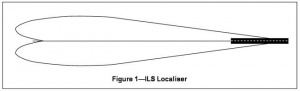
\includegraphics[width=0.4\textwidth, trim={0.2cm 0.5cm 0.2cm 0.1cm}, clip]{img/ILS-LOC}}
	\caption{Rà dio localitzador ILS}
	\label{fig-ils-loc}
\end{figure}

L'altra ràdio és la de pendent de descens o \textit{Glide-Scope} (GS), que permet a
l'aeronau controlar la ràtio de descens durant l'aproximació. (la figura \ref{fig-ils-gs} mostra la
pista d'aterratge i la senyal de ràdio vistes de perfil).

\begin{figure}[!h]
\centering
\fbox{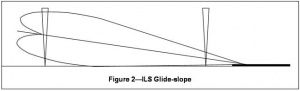
\includegraphics[width=0.4\textwidth, trim={0.2cm 0.5cm 0.2cm 0.1cm}, clip]{img/ILS-GS}}
	\caption{Ràdio Glide-Scope ILS}
	\label{fig-ils-gs}
\end{figure}

El sistema ILS funciona bé i és molt robust, però necessita que les antenes de ràdio
a la pista estiguin instal·lades i funcionin correctament, i avui en dia només els
aeroports i aeròdroms amb més trànsit solen tenir aquest sistema, les pistes més petites i els aeròdroms en llocs remots solen quedar fora de l'equació pel que fa a aterratges
amb ILS.

% ######################### DIAGRAMA DE GANTT ############################
\definecolor{barblue}{RGB}{153,204,254}
\definecolor{groupblue}{RGB}{51,102,254}
\definecolor{linkred}{RGB}{165,0,33}
\renewcommand\sfdefault{phv}
\renewcommand\mddefault{mc}
\renewcommand\bfdefault{bc}
\setganttlinklabel{s-s}{}
\setganttlinklabel{f-s}{}
\setganttlinklabel{f-f}{}
\sffamily
\begin{figure*}
\begin{ganttchart}[
    y unit chart=.75cm,
    canvas/.append style={fill=none, draw=black!5, line width=.75pt},
    hgrid style/.style={draw=black!5, line width=.75pt},
    vgrid={*1{draw=black!5, line width=.75pt}},
    today label font=\small\bfseries,
    title/.style={draw=none, fill=none},
    title label font=\bfseries\footnotesize,
    title label node/.append style={below=7pt},
    include title in canvas=false,
    bar label font=\mdseries\small\color{black!70},
    bar label node/.append style={left=2cm},
    bar/.append style={draw=none, fill=black!63},
    bar incomplete/.append style={fill=barblue},
    bar progress label font=\mdseries\footnotesize\color{black!70},
    group incomplete/.append style={fill=groupblue},
    group left shift=0,
    group right shift=0,
    group height=.5,
    group peaks tip position=0,
    group label node/.append style={left=.6cm},
    group progress label font=\bfseries\small,
    link/.style={-latex, line width=1.5pt, linkred},
    link label font=\scriptsize\bfseries,
    link label node/.append style={below left=-2pt and 0pt}
  ]{1}{19}
  \gantttitle[
    title label node/.append style={below left=7pt and -3pt}
  ]{Setmanes:\quad1}{1}
  \gantttitlelist{2,...,19}{1} \\
  
  % 1 ----------------------------------------------------------
  \ganttgroup[progress=100]{1.Planificar el projecte}{1}{4} \\
  
  % 2 ----------------------------------------------------------
  \ganttgroup[progress=100]{2.Investigar possibles solucions}{1}{4} \\
  \ganttbar[
    progress=100,
    name=WBS2A
  ]{\textbf{2.1} Recopilar possibles solucions}{1}{2} \\
  \ganttbar[
    progress=100,
    name=WBS2B
  ]{\textbf{2.2} Investigar pros i contres}{3}{3} \\
  \ganttbar[
    progress=100,
    name=WBS2C
  ]{\textbf{2.3} Escollir models}{4}{4} \\
  
  % 3 ----------------------------------------------------------
  \ganttgroup[progress=100]{3. Implementar solucions per a una sola pista}{5}{10} \\
  \ganttbar[
    progress=100,
    name=WBS3A
  ]{\textbf{3.1} Crear dataset}{5}{6} \\
  \ganttbar[
    progress=100,
    name=WBS3B
  ]{\textbf{3.2} Implementar algoritme d'entrenament}{7}{9} \\
  \ganttbar[
    progress=100,
    name=WBS3C
  ]{\textbf{3.3} Provar model}{10}{10} \\
  
  % 4 ----------------------------------------------------------
  \ganttgroup[progress=100]{4.Implementar simulació completa}{1}{3} \\
  \ganttbar[
    progress=100,
    name=WBS4A
  ]{\textbf{4.1} Recopilar possibles solucions}{1}{1} \\
  \ganttbar[
    progress=100,
    name=WBS4B
  ]{\textbf{4.2} Implementar simulació de terreny}{2}{3} \\
  \ganttbar[
    progress=100,
    name=WBS4C
  ]{\textbf{4.3} Implementar simulació avió}{2}{3} \\
  
  % 5 ----------------------------------------------------------
  \ganttgroup[
    progress=100,
    name=5
  ]{5.Provar model sobre la simulació i ajustar-lo}{11}{12} \\
  
  % 6 ----------------------------------------------------------
  \ganttgroup[
    progress=100,
    name=6
  ]{6.Investigar integració arduino amb avió rc}{1}{1} \\
  
  % 7 ----------------------------------------------------------
  \ganttgroup[
    progress=30
  ]{7.Crear avió pathfinder}{1}{9} \\
  \ganttbar[
    progress=100,
    name=WBS7A
  ]{\textbf{7.1} Investigar sobre avions radiocontrol}{1}{2} \\
  \ganttbar[
    progress=10,
    name=WBS7B
  ]{\textbf{7.2} Construir estructura principal}{3}{4} \\
  \ganttbar[
    progress=80,
    name=WBS7C
  ]{\textbf{7.3} Construir electrònica del model}{5}{7} \\
  \ganttbar[
    progress=0,
    name=WBS7D
  ]{\textbf{7.4} Proves inicials de vol}{8}{9} \\
  
  % 8 ----------------------------------------------------------
  \ganttgroup[
    progress=0
  ]{8.Construir avió definitiu}{10}{12} \\
  \ganttbar[
    progress=0,
    name=WBS8A
  ]{\textbf{8.1} Construir estructura principal}{10}{10} \\
  \ganttbar[
    progress=0,
    name=WBS8B
  ]{\textbf{8.2} Construir electrònica del model}{11}{11} \\
  \ganttbar[
    progress=0,
    name=WBS8C
  ]{\textbf{8.3} Integrar hardware}{12}{12} \\
  
  % 9 ----------------------------------------------------------
  \ganttgroup[
    progress=0,
    name=9
  ]{9.Implementar Xarxa Neuronal en el model}{13}{13} \\
  
  % 10 ----------------------------------------------------------
  \ganttgroup[
    progress=0
  ]{10.Provar model sobre una pista d'aterratge real}{14}{15} \\
  \ganttbar[
    progress=0,
    name=WBS10A
  ]{\textbf{10.1} Sobrevolar}{14}{14} \\
  \ganttbar[
    progress=0,
    name=WBS10B
  ]{\textbf{10.2} Ràfagues curted de vol autònom}{14}{14} \\
  \ganttbar[
    progress=0,
    name=WBS10C
  ]{\textbf{10.3} Aproximacions completes}{15}{15} \\
  \ganttbar[
    progress=0,
    name=WBS10D
  ]{\textbf{10.4} Aterratge complet}{15}{15} \\
  
  % 11 ----------------------------------------------------------
  \ganttgroup[
    progress=0,
    name=11
  ]{11.Ampliar la xarxa neuronal}{16}{17} \\
  
  \ganttlink[link type=f-s]{WBS2A}{WBS2B}
  \ganttlink[link type=f-s]{WBS2B}{WBS2C}
  
  \ganttlink[link type=f-s]{WBS2C}{WBS3A}
  \ganttlink[link type=f-s]{WBS3A}{WBS3B}
  \ganttlink[link type=f-s]{WBS3B}{WBS3C}
  
  \ganttlink[link type=f-s]{WBS4A}{WBS4B}
  \ganttlink[link type=f-s]{WBS4A}{WBS4C}
  
  \ganttlink[link type=f-s]{WBS3C}{5}
  \ganttlink[link type=f-s]{WBS4C}{5}
  
  \ganttlink[link type=f-s]{WBS7A}{WBS7B}
  \ganttlink[link type=f-s]{WBS7B}{WBS7C}
  \ganttlink[link type=f-s]{WBS7C}{WBS7D}
  
  \ganttlink[link type=f-s]{WBS7D}{WBS8A}
  \ganttlink[link type=f-s]{WBS8A}{WBS8B}
  \ganttlink[link type=f-s]{WBS8B}{WBS8C}
  
  \ganttlink[link type=f-s]{WBS8C}{9}
  
  \ganttlink[link type=f-s]{9}{WBS10A}
  \ganttlink[link type=s-s]{WBS10A}{WBS10B}
  \ganttlink[link type=f-s]{WBS10B}{WBS10C}
  \ganttlink[link type=s-s]{WBS10C}{WBS10D}
  
  \ganttlink[link type=f-s]{WBS10D}{11}
  
  \ganttlink[link type=f-s]{5}{9}
  
  \ganttvrule{Informe 1}{4}
  \ganttvrule{Progrés(I)}{9}
  \ganttvrule{Progrés(II)}{14}
  \ganttvrule{Final}{17}
  
  
\end{ganttchart}
\caption{Diagrama de Gantt del projecte}
\label{fig-gantt}
\end{figure*}

\Needspace{10\baselineskip}

\section{Desenvolupament}
He actualitzat el diagrama de Gantt (figura \ref{fig-gantt}) per mostrar el progrés del projecte fins al moment, i s'hi pot veure que les tasques
de la 1 a la 6 estan completades. Tenint en compte que les tasques entre la 1 i la 5 representen el desenvolupament complet del meu
Minimum Viable Product tal i com està estipulat en els meus objectius, considero que el meu progrés en les últimes setmanes ha estat
molt adequat i que el meu TFG es podria donar per finalitzat en el seu estat actual de forma satisfactòria, si així fos necessari.

En les pròximes seccions detallaré el progrés que he fet fins al moment. En aquells punts que ja vaig comentar en l'informe actualitzaré
la informació on sigui necessari, i afegiré els punts nous que he desenvolupat desde llavors.
\subsection{Tasca 2: Investigar possibles solucions}
Al principi del projecte es van plantejar varis models d'aprenentatge per a la detecció de la pista, i sobretot se'n van discutir més en profunditat tres:
\begin{itemize}
    \item{Detectors de característiques de l'estil de Sift o Surf \cite{khan2011sift}, són molt ràpids però tenen dificultats detectant característiques complexes en totes les condicions possibles.}
    \item{Detectors de segmentació semàntica, principalment U-Net \cite{ronneberger2015u}, pot ser més lent però és flexible i pot donar prediccions fiables en entorns molt complexos.}
    \item{Entrenament End-to-End \cite{bojarski2016end}, on la intenció és que una sola xarxa neuronal resolgui el problema de visió i el de control alhora. Pot donar molt bons resultats però és més difícil d'entrenar correctament.}
\end{itemize}

Finalment he continuat el projecte amb un detector de segmentació semàntica, que consisteix en una xarxa neuronal que rep com a input una imatge
i retorna una màscara que separa les parts de la imatge que són pista d'aterratge i les que no ho són (figura \ref{fig-img-seg-exmpl}).

\begin{figure}[h]
\centering
\fbox{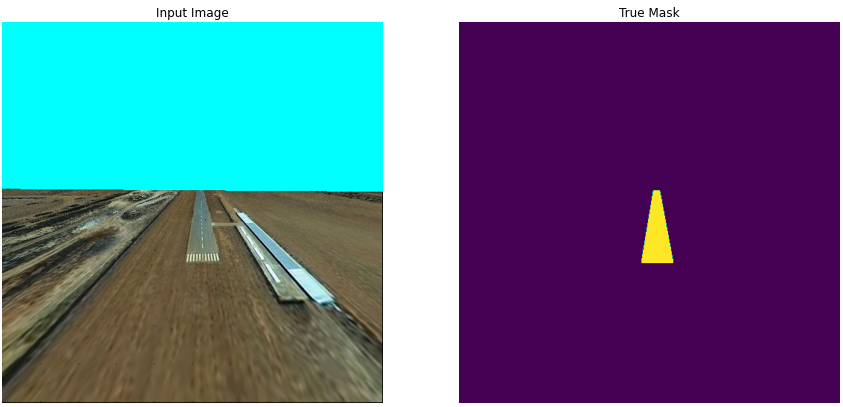
\includegraphics[width=0.4\textwidth]{img/TrueMaskExample}}
    \caption{Exemple d'una imatge i la predicció esperada}
    \label{fig-img-seg-exmpl}
\end{figure}

\subsection{Tasca 3: Implementar la solució escollida}
Aquest apartat és el que ha vist més progrés en les últimes setmanes. Un cop escollit el model d'entrenament em calia trobar una forma de generar
la gran quantitat d'imatges requerides per a entrenar un model de segmentació semàntica. Volia un sistema d'aprenentatge no supervisat que pogués
generar models i datasets d'inici a fí sense input humà, perquè el temps que tinc és limitat i no em puc dedicar a anotar imatges, i perquè 
l'escalabilitat d'un sistema no supervisat és molt més senzilla i directa.

He montat un sistema que genera homografies d'imatges satèl·lit per generar una sensació de perspectiva que considero que serà suficient per entrenar
un model, i només necessita les coordenades de les quatre cantonades de la pista d'aterratge per fer-ho
(de l'estil de les imatges en la figura \ref{fig-img-seg-exmpl}).
I com que conec les cordenades de la pista d'aterratge i les seves cantonades puc generar la màscara automàticament també.

Un cop tinc la imatge del terreny generada he afegit un procés que distorsiona la imatge només a la part que correspon al terra, amb la intenció
d'evitar que una xarxa neuronal pogués aprendre a reconèixer les homografies de les pistes utilitzades en el dataset, i d'aquesta manera
evitar l'overfitting de la xarxa. Afegir aquest pas ha donat molt bons resultats i les xarxes que he pogut entrenar generalitzen molt millor
quan es troben amb imatges del món real.

Tot i així, només puc generar una imatge cada 2 segons més o menys, ja que cada imatge fa unes 100 crides asíncrones al servei d'imatges satèl·lit i estic
limitat pel major temps de resposta, per tant també he implementat un sistema d'augmentació de dades que fa zoom en diferents posicions de cada
imatge i extreu unes 120 imatges noves per a cada imatge original.

Un cop s'han generat les imatges es passen automàticament per l'entrenament de la xarxa neuronal, amb resultats adequats al punt de progrés en que
em trobo actualment(figura \ref{fig-pred-exmpl}).

En les últimes setmanes he experimentat amb models que puguin reconèixer el cel i la pista, en comptes de només la pista, amb resultats que
no han estat ben bé els esperats. Els models funcionen bé, però no queda clar encara que aportin millora respecte els models que detecten
només la pista, i per l'arquitectura i algoritme de control que he implementat no és necessaria la detecció del cel.

Tot l'entrenament l'he fet en Google Colab perque m'ha donat millors resultats, així que el codi a Github no està sempre actualitzat.
Es pot veure el codi més recent en el que estic treballant \href{https://colab.research.google.com/drive/1fX-1lhTc6W_ACkCkY24vqCnT4GJXCWct?usp=sharing}{aquí}.

\begin{figure}[h]
\centering
\fbox{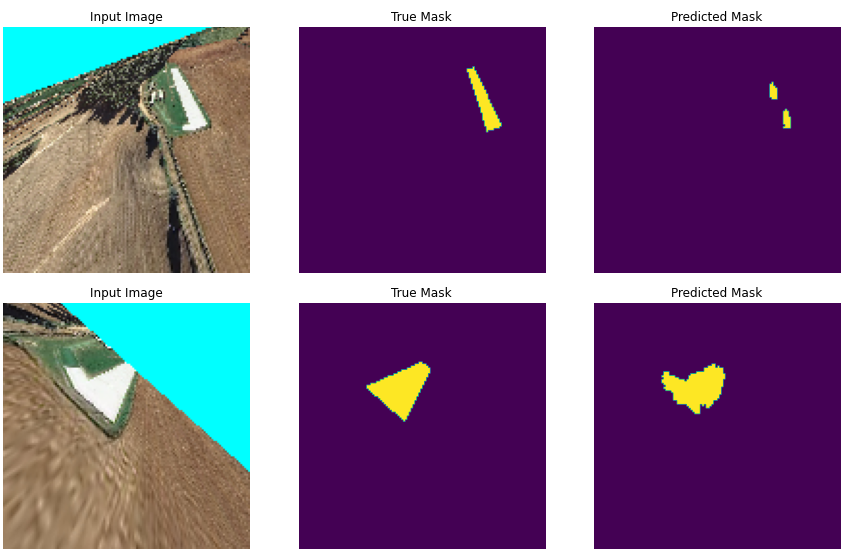
\includegraphics[width=0.4\textwidth]{img/PredictionsExample}}
    \caption{Dues imatges, les seves prediccions esperades i les prediccions reals}
    \label{fig-pred-exmpl}
\end{figure}

\subsection{Tasca 4: Implementar una simulació completa}
Per a aquesta tasca vaig decidir utilitzar el motor de creació de videojocs Unity per a fer la simulació d'un avió, un terreny i una pista
d'aterratge (figura \ref{fig-simulador}). També vaig implementar un motor físic per a simular el moviment de l'avió segons la pisició de les seves
vàries superfícies de control.
\begin{figure}[h]
\centering
\fbox{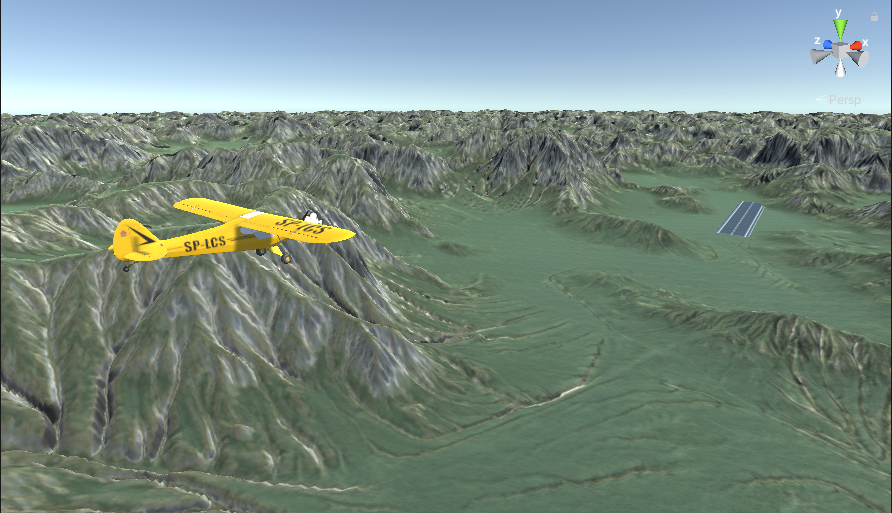
\includegraphics[width=0.4\textwidth]{img/Simulador}}
    \caption{Simulació de l'avió i la pista d'aterratge}
    \label{fig-simulador}
\end{figure}

Per a provar el meu sistema de control autònom sobre el simulador necessitava una forma de controlar Unity amb Python, i com que Unity no suporta
Python directament he montat un programa de control en Python que es comunica amb el controlador de l'avió a Unity per Sockets. La idea és que
pugui rebre la imatge que captura la càmera de l'avió simulat (figura \ref{fig-simulador-controlador}), processar-la i enviar les posicions de les superfícies de control que considera
necessàries.

\begin{figure}[h]
\centering
\fbox{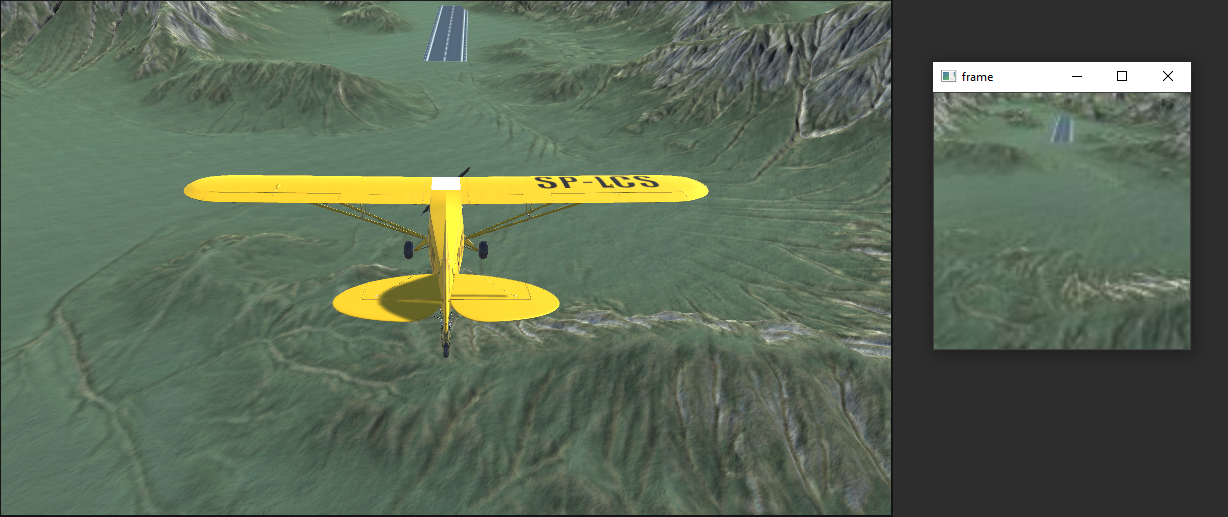
\includegraphics[width=0.4\textwidth]{img/SimuladorIControlador}}
    \caption{Simulador a l'esquerra i la imatge rebuda pel controlador a la dreta}
    \label{fig-simulador-controlador}
\end{figure}

\subsection{Tasca 5: Integració del model i la simulació i programar el control de l'avió}
Un cop implementat el simulador i una xarxa neuronal que generalitzi bé he dedicat les últimes setmanes a integrar-los tots
dos, de manera que el servidor en python pugués veure l'estat del simulador, analitzar-lo utilitzant els models entrenats
prèviament i diferents tècniques d'anàlisi d'imatges, i enviar una resposta al simulador per poder controlar l'avió, tot
tant en temps real com fos possible. Desde instal·lar i provar diferents configuracions de drivers de Nvidia i versions
de les diferents llibreries que utilitzo fins a utilitzar multithreading per separar la comunicació amb el simulador i 
l'anàlisi pròpiament dit, finalment tot el bucle funciona 10 vegades cada segon, que és més que suficient per el que necessito.

Per analitzar una imatge el primer que faig és fer una predicció de segmentació semàntica amb la xarxa neuronal per obtenir 
una aproximació del que és la pista i el cel, després extrec només una màscara per la pista i la erosiono i la dilato
seqüencialment per eliminar el soroll. Com que normalment no s'elimina tot el soroll assumeixo que el bloc més gran és la
pista i en busco el punt mig i els punts màxims i mínims per trobar les cantonades. Finalment busco el punt mig de l'aresta
de la pista més propera a l'avió, ja que aquest punt és el que servirà de referència per al controlador a l'hora de dirigir
l'avió.

Per la banda del controlador, llavors, cada dècima de segon arriba un punt representat per dues coordenades, i que representa
el centre de l'aresta més pròxima de la pista en el pla en dues dimensions que veu la càmera frontal de l'avió. Com que 
conec la posició de la càmera i l'angle actual de l'avió (recordo que l'avió incorpora un giroscopi), puc traduïr aquestes
coordenades en un vector que indica la direcció i el sentit cap a la pista desde l'avió. Aquest vector és el que es seguirà
fins que arribi el següent frame i es repeteixi el procés. Per eliminar soroll, cal remarcar que en realitat el vector es
calcula amb la mitjana dels deu últims punts que han arribat, ja que com que el moviment de l'avió no és brusc un delay de 
aproximadament un segon no impossibilita un bon resultat i ajuda molt en reduïr moviments bruscs per punts que no han
estat ben detectats en algun frame.

\subsection{Tasca 6: Investigar integració arduino amb radiocontrol}
Aquesta és la última secció que vull destacar. El meu tfg també inclou en els seus objectius opcionals construir un avió a escala i aconseguir
que aterri automàticament, així que he estat investigant la manera de construïr un avió que tingui la programabilitat suficient per a donar-me
la flexibilitat que vull, la potència de càlcul suficient per a fer anar la xara neuronal i tots els càlculs necessaris a un framerate suficient
i que es pogués integrar amb un transmissor i un receptor radiocontrol convencionals.

Finalment he acabat amb un sistema que consisteix en un arduino micro com a controlador dels servos i el motor, una raspberry pi zero o 
una Jetson Nano per al reconeixement de la pista i el control autònom, un Taranis Q X7 per al transmissor radiocontrol i un Taranis R-XSR
per al receptor radiocontrol, tots dos de la marca FrSky. He escollit Taranis perquè la majoria dels productes són de codi obert i permeten
comunicació bidireccional, de manera que els podria programar per rebre telemetria de l'avió directament al transmissor i saber a temps real
l'estat dels algoritmes autònoms i la confiança del controlador en un bon aterratge.


% BIBLIOGRAFIA --------------------------------------------------------
\bibliographystyle{apacite}
\bibliography{mybib}

\end{document}
